\begin{SCfigure}[2\sidecaptionrelwidth][ht]
	\centering
	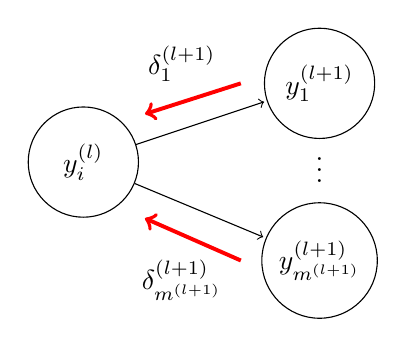
\begin{tikzpicture}[shorten >=1pt]
      		\tikzstyle{unit}=[draw,shape=circle,minimum size =1.4cm]
 
       	\node[unit](i) at (0,1){$y_i^{(l)}$};
        	\node[unit](k1) at (3,2){$y_1^{(l+1)}$};
		\node at (3, 1){$\vdots$};
		\node[unit](km) at (3,-0.25){$y_{m^{(l+1)}}^{(l+1)}$};
		
		\node at (1.25,2.25){$\delta_1^{(l+1)}$};
		\node at (1.25,-0.5){$\delta_{m^{(l+1)}}^{(l+1)}$};
 
        	\draw[->] (i) -- (k1);
		\draw[->] (i) -- (km);
		
		\draw[->,red,line width=0.05cm] (2,-0.25) -- (0.75,0.3);
		\draw[->,red,line width=0.05cm] (2,2) -- (0.75,1.6);
    	\end{tikzpicture}
	\caption[Backpropagation.]{\small{Backpropagation of errors through the network; once evaluated for all output units, the errors $\delta_i^{(L+1)}$ can be propagated backward.}}
	\label{fig:error-backpropagation}
\end{SCfigure}